\documentclass[12pt,a4paper,twoside]{report}

\usepackage[lmargin=2.54cm,tmargin=2.54cm,rmargin=2.54cm,bmargin=2.52cm]{geometry}
\usepackage[utf8]{inputenc}
\usepackage[T1]{fontenc}
%\usepackage{cite}

\usepackage{mathptmx}
\usepackage{fancyhdr}
\usepackage{graphicx}
\usepackage{subcaption}
\usepackage{pdfpages} 
\usepackage{amsmath}
%\usepackage{showframe}
%\usepackage[citestyle=alphabetic,bibstyle=authortitle]{biblatex} 
%\addbibresource{ProjectResearchPapers.bib}

\pagestyle{fancy}
\fancyhf{}
\fancyhead[LE,RO]{The University of Sheffield}
\fancyhead[RE,LO]{Akinola Alexander Dada}
\fancyfoot[CE,CO]{\thepage}
\fancyfoot[LE,RO]{Master's Dissertation}
\fancyfoot[RE,LO]{ACSE}

\linespread{1.5}

\title{ Modelling, Simulation, and Implementation of Linear Control for Asymmetric Multirotor Unmanned Aerial Vehicles}
\author{Akinola Alexander Dada \\ Reg No.160140802}
\date{$\today$}

\begin{document}
		
	\maketitle
	
	\newpage
	
	\tableofcontents
	
	\newpage
	
	\listoffigures
	
	\newpage
	
	\listoftables
	
	\newpage
	
	\begin{abstract}
		Unmanned Aerial Vehicles (UAVs) are aerial systems not directly controlled by onboard personnel. There are many types of UAV platforms, chiefly defined by the characteristics of their mechanical construction. One such class of UAVs are multirotors which possess multiple rotor wing actuators. These types of UAVs have a wide range of applications due to their ability to perform vertical/Short take-off and landing (VSTOL), stationary and low speed flight, coupled with their relatively simple mechanical designs when compared to single rotor constructions, such as more traditional helicopters. The major challenge in dealing with these types of UAVs is their inherent instability in flight, save for the intervention of complex control systems. Therefore, in order to understand control systems capable of producing guaranteed requirement meeting performance, this project first seeks to investigate the physical characteristics and responses of UAVs through mathematical modelling, then proceeds to, design, develop, implement and compare the performance of 2 advanced linear control schemes on an embedded microprocessor, where this level of insight is requisite. These control schemes are, Linear Quadratic Gaussian (LQG) and Linear Quadratic Model Predictive Control (LQ-MPC). 
	\end{abstract}
	\newpage
	
	\section*{Executive Summary}
		This report documents the steps undertaken in the investigation of asymmetric multirotor UAV characteristics, as well as a walkthrough of the processes involved in using those characteristics to guide and inform the design, development and implementation of linear feedback control systems which are capable of providing guaranteed performance.
		\\ \\
		The first section provides a project introduction containing background information pertinent to the investigation, briefly discussing the nature and potential uses of UAVs. This section includes the systems engineering approaches taken, such as breaking down the project aims and objectives and setting them up as a set of task requirements with achievable milestones. This section provides information on project planning and management which includes the use of Gantt charts amongst others. This section will also detail all considerations and changes made to the project due to the SARSCOVID-2 pandemic.
		\\ \\
		The second section reviews and provides an analysis of the relevant supporting literature collected, which is referenced throughout the writing. The supporting research materials take the form of scientific journals articles, independent research publications, exerts from university lectures, Master’s/ PhD thesis publications and published books.
		\\ \\
		The third section briefly discusses the mechanical design and construction of the specific asymmetric Y6 ‘hexarotor’ UAV being used as the case study. This Section goes through and details the processes and results of analysing the UAV and deriving a mathematical representation of the physical characteristic through a combination of first principles dynamic modelling and hardware-in-the-loop (HIL) testing. This section explores and expatiates on different modelling techniques while discussing the various assumptions made during the modelling process and the reasoning behind the adopting of the techniques chosen. This section then converts the derived model into various forms useful for control design, analysis and simulation while presenting rigorous analyses of the system characteristics along with a dynamic simulation using industry standard applications.
		\\ \\
		The forth section details the process behind the design and development of an LQG feedback controller, then discusses and analyses the simulation results. This section then discusses the limitations of LQG controllers. This section details the design and development of LQ-MPC feedback controllers. Extending from the previous section, this section presents and justifies the reasoning behind transitioning to LQ-MPC as well as analysing the simulation results of the LQ-MPC feedback controller. This section then compares the performance of the LQG and LQ-MPC feedback controllers using appropriate metrics.
		\\ \\
		The fifth section discusses the characteristics of the embedded Linux single board computers (SBCs), using the BeagleBone Blue platform. This section discusses and details the processes and considerations behind implementing UAV control systems on the platform. The section then presents a Unified Modelling Language (UML) Class diagram detailing an implementation proposal for an embedded LQG Controller in the C Language.
		\\ \\
		The sixth and final section concludes the report and presents possibilities for future work and development.
		
	\newpage
	
	\section{Introduction}
		
		\begin{enumerate}
			\item
				Background.
			\item 
				Aims and Objectives. 
			\item 
				Project Management.
		\end{enumerate}
	
	 	\newpage
	 	
		\subsection{Background}
		
			UAVs are aerial systems which are not directly controlled by a human onboard the vehicle. There are many types of UAV platforms which are chiefly defined by the characteristics of their mechanical constructions [3][4]. These defining criteria break down to include:
			
			\begin{itemize}
				\item
					The position, number and type of their actuators.
				\item 
					Their mode/modes of flight. 
				\item 
					Their use cases specific features.
			\end{itemize}
			\space
			One such type of UAVs are multirotors, defined as such due to their multiple rotor wing actuators. UAVs of this description were developed in response to the mechanical complexity of single or dual rotor winged aircraft such as the various helicopter and auto-gyros variants. The greater simplicity of multirotor craft could potentially lead to reduced development, construction and maintenance costs as well as greater reliability in use. Both classes of UAVs possess the ability to perform operations requiring VTOL, stationary and low speed flight [12].
			\\
			These features enable them to be utilised in many wide ranging applications, where great dexterity in motion is required, and as such would not be possible using fixed winged platforms, such as operations required during; directed precision administration of substances to plants in precision agriculture, frequent and or detailed inspection of standing structures, precision wide area surveillance, amongst many others [6].
			\\
			However, the major challenge in dealing with multirotor UAVs is their inherent instability in real world flight situations, where disturbances are present, making it impossible to operate these craft with direct open loop control of their actuators, as is possible and frequently done with fixed winged craft. Therefore, the need for the development of control systems is apparent. 
			\\
			In order for the developed control systems to behave in a guaranteed predictable manner and be able to meet defined performance specifications, it becomes necessary to understand the behaviour of the system to be controlled and thus derive a mathematical behavioural representation to be used in guiding and informing the design process, which is done through mathematical systems modelling. This level of insight is also required in the development of advanced control schemes.
		
		
		\subsection{Aims and Objectives}
			
			The framework of this project was set around the design and development of control software for VSTOL model aircraft. From this broad theme, the aims of modelling an asymmetric multi-rotor platform, developing multiple control schemes and then implementing these schemes on a multirotor platform via an embedded SBC were derived.
			\\
			These aims break down into multiple objectives and milestones which must each be achieved to fulfil the full scope of the aims outlined. These objectives can be broadly classified into 2 categories: 
	
				\subsection*{Basic Objectives}
				
					\begin{enumerate}
						\item
							Develop a mathematical model representing the dynamics of the multirotor aircraft.
						\item
							Develop a dynamic simulation of the crafts behaviour.
						\item
							Develop LQG feedback control.
						\item
							Investigate feedback control laws in simulation with the mathematical model to achieve behavioural targets.
						\item
							Develop flight control software to interface with sensors and implement control laws.
						\item
							Implement the flight control software on an embedded microprocessor unit(**).
						\item
							Discuss the results of performance comparisons between the simulation and hardware implementations(**).
					\end{enumerate}
				
				\subsection*{Advanced Objectives}
				
					\begin{enumerate}
						\item
							Investigate the application of LQ-MPC schemes in simulation.
						\item	
							Incorporate and implement LQ-MPC schemes unto the flight control software(**).
						\item	
							Discuss the differences between the LQG and LQ-MPC implementations.
					\end{enumerate}
				
		\subsection{Project Management}
			
			\begin{figure}[h!]
				\centering
				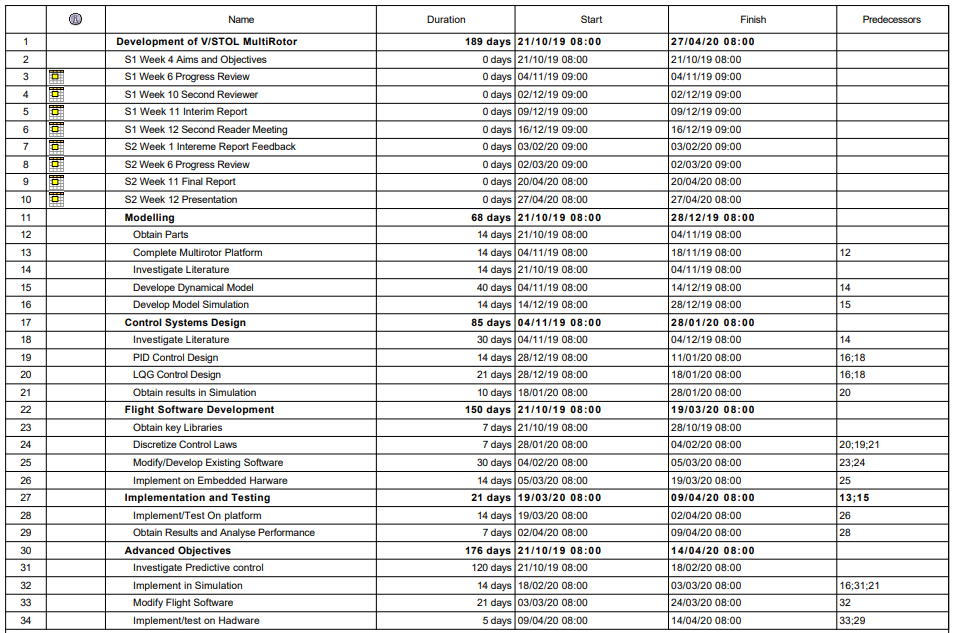
\includegraphics[width=1.1\linewidth]{ProjectInitialTimetable.png}
				\caption{Initial Timetable}
				\label{fig:initialtimetable}
			\end{figure}
		
			\begin{figure}[h!]
				\centering
				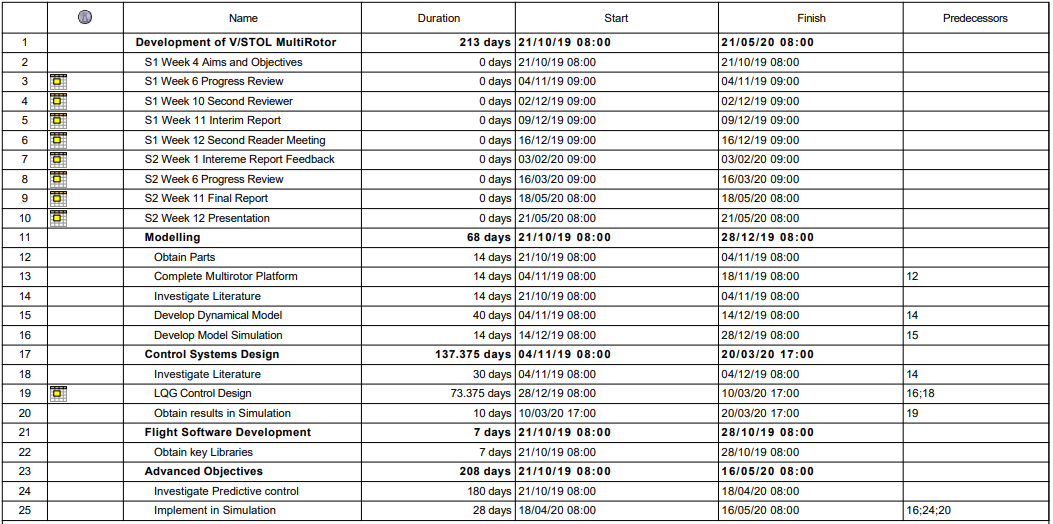
\includegraphics[width=1.1\linewidth]{ProjectFinalTimetable.png}
				\caption{Final Timetable}
				\label{fig:finaltimetable}
			\end{figure}
		
			In order to properly execute on the project Aims and Objectives, project activities were coordinated and managed by further breaking down or grouping task then laying them out in tabulations which were used to generate the project Gantt charts.
			\\
			The project has by in large proceeded along on the initial schedule proposed with only one major non SARSCOVID-2 related change made to tasks and execution dates from the initial proposal. 
			\\ \\
			Due to the effects and responses to the global SARSCOVID-2 pandemic, which first emerged in Wuhan city China in late November of 2019, The University of Sheffield was forced into closure/Cancellation of all on-site and in-person teaching, meetings and instruction from March of 2020. This coupled with the government mandated nationwide quarantine and lockdown in the United Kingdom made access to the necessary facilities for the testing and evaluation of any developed UAV software impossible. As such, activities and work towards meeting the objectives succeeded by a double Asterix in the previous subsections is not being undertaken. Project planning has been adjusted accordingly. This has also led to changes in term dates which resulted in adjustments being made to task timelines.
			\\ \\
			All material purchases were made on time, acquiring key hardware such as the main flight computer, the flight radio control system, which would have served as the main communication unit sending control commands to the multirotor, electronics speed controllers, and load cells which will be used to develop the lab-bench platforms to identify the actuator dynamics. All Ad hoc minor changes to task completion periods are reflected in timeline changes from the initial proposal table to the final proposal table. 
			\\
			The only non SARSCOVID-2 enforced change in the project from its initial proposal was the dropping of a PID control design section which occurred before, and is reflected in, the S2 week project proposal review. This change was made to refocus the project objectives solely on model-based control design outcomes.
			\\ \\
			All changes to task completion dates for further objectives are displayed in the final proposal table which was used to produce the final full project Gantt chart available in the Appendix.
			
	\newpage
	
	\section{Review Of Literature }	
	
		In preparing to execute the project tasks, various supporting and reference materials were acquired. The various literature take the form of articles published in scientific journals, research publications, exerts from university lectures, Masters and PhD thesis publications and published books, all of which together broadly cover and present 3 major themes that are relevant to the project’s investigation:
		
		\begin{enumerate}
			\item 
				Mathematical Modelling and Systems Identification. 
			\item 
				Control Systems Design.
			\item 
				Simulation and Implementation.
		\end{enumerate}
	
		\newpage
		
		\subsection{Mathematical Modelling and System Identification}
			
			\subsection*{UAV}
				
				The UAV is actuated by 6 1000Kv brushless direct current (BLDC) motors [14], attached to 6 10x45inch propellers and is powered by a 4-cell lithium-polymer battery with an operational voltage range of 16.8 volts to 12.8 volts. The UAV has dimensions of, 45 cm in length from rear motor centres to from motor centres, 44 cm in length from left motor centres to right motor centres, and a mass of 1.3 kilograms. The exact details involved with the design, development and construction of UAVs is beyond the scope of the project investigation but material, mechanical and electronic consideration when designing such craft are explored in [12].
				
			\subsection*{Dynamics}
				In modelling systems, it is first necessary to state all assumptions made about its characteristics. These assumptions simplify the process of systems model abstraction to ensure minimum viability standards are met. Following that, multirotors can be defined as rigid-bodies free to move in three-dimensional (3-D) space, therefore, they move with 6 degrees of freedom (6-DOF). With this modelling assumption, the motion of the vehicles is subject to the laws of rigid body Kinematics and Kinetics. All the acquired material takes this stance. 
				\\
				Vehicle motion is defined in terms of 2 coordinate frames moving relative to one another where the physical quantities that change with time, states, change with respect to one frame or the other. They are the Earth-Frame, fixed to the earth and the Body-Frame, attached to the vehicle body. Each frame consists of 3 orthogonal axes, whose nomenclature varies from source to source, about and along which rotational and translational motion can occur respectively [1][2][4][15]. 
				\\
				The sources obtained explore 2 ways for representing this rotational motion of the reference frames:
				
				\begin{itemize}
					\item 
						Sources [1][2][3][4][5][6][7][9] present their models using Euler angles which describe arbitrary orientation in the 3-dimensional Euclidean space using three parameters which represent a sequence of three elemental rotations about each axes of the coordinate system. Any orientation in 3D space can be achieved by composing these 3 elemental rotations.
					\item
						Sources [1][8][16] present representations through Quaternions which solve issues present with computing Euler angles such as computational expense and numerical singularities which occur when certain orientations are reached, as it does not require the calculation of sin and cos when certain angles go to 0 or 90 degrees and their multiples. Quaternions represent any arbitrary orientation by constructing rotations as that of a single angle about an imaginary axis. 
				\end{itemize}
				\space
				The rigid body assumptions also allow for the utilisation of several Mechanical Modelling techniques and conventions which are used to derive the non-linear dynamics of the body frame mechanical systems considering both kinematics and Kinetics:
				
				\begin{itemize}
					\item
						The Newton-Euler convention which derives representations of systems dynamics through the application of first principles using newtons 2nd law of motion showing the effects of forces applied to the rigid body by its actuators and environment. utilised in [2][3][5][6][7][8][9]
					\item 
						The Euler-Lagrange convention which derives representations of systems dynamics through the study of energy differentials between kinetic and gravitational potential generated by motion. utilised in [4]. 
					\item 
						The Newton-Hamiltonian.
					\item 
						Pure Hardware-in-the-Loop system identification, which decouples each axes of motion and determines approximate model frameworks for each then populates said framework with experimentally obtained elements. such was the process taken by [30]
				\end{itemize}
				\space
				This investigation utilises the Euler-angle representation and the Newton-Euler convention due to its intuitive familiarity and relative simplicity.
				\\
				Due to the UAV's layout, it is asymmetric, this creates a system where its mass is not geometrically evenly distributed about the centre of mass leading to where inertia is not represented by a diagonal inertial tensor but instead one with non-trivial off diagonal elements and thus creating transposed reference frames. However, for the purpose of this investigation, it is assumed that the system is symmetrical as the off-diagonal terms in the inertia matrix are far lower in magnitude than the diagonal terms, thus can be reasonably neglected. Otherwise, the entire coordinates system would be adjusted and transformed to produce a true diagonal matrix as presented in [10]. 
				\\ \\
				In order to design the controllers, the non-linear model obtained via the Newton-Euler convention needs to be linearised. This is accomplished through the application of Jacobi’s linearisation method as presented in [11]. This process produces a full linear state space representation of systems dynamics around stable operating points. This model is then discretized for implementation in digital embedded systems.
				
			\subsection*{Actuator Dynamics}	
				As stated in the UAV subsection, the multi-rotor is actuated by BLDC motors [14], To fully develop a system model, these must be modelled. This can either be done via first principles calculations as presented in [2][8][17] or via experimental systems identification as presented in [9][12][14][15][16]. 
				\\
				The systems identification approach involves the derivation of a lumped parameter linear input- output model, encompassing the electronic speed control unit, motor and propeller dynamics, between input Pulse width modulated (PWM) signal duty cycles or pulse width and the output angular velocity, torque and thrust forces. This has the advantage of reducing complex dynamics enabling the utilisation of a minimum viable model and as such, is being implemented in this investigation.
				
		\subsection{Control Systems Design, Simulation and Implementation}
		
			\subsection*{LQG}
				The Linear Quadratic Gaussian makes use of the full state of a system, obtainable from a limited set of measurements through the application of a Gaussian estimator, in this case a Kalman filter[23][24][25][26], to obtain the full state. It is a form of optimal control where its objective is to find a set of control actions which minimize some cost or performance function to bring the system’s state to a desired set of values. Sources [18][19][21][22][31] present derivations of state feedback control leading to different implementation of LQG control. Source [20] details implementation of LQG control in embedded systems.
				
			\subsection*{LQ-MPC}
				Like LQG, MPC is also a kind of optimal control, however, this technique’s cost or performance function is limited to looking at future states over some fixed finite horizon and control signals can be determined so that they implicitly taking into account and determine control action so as to meet physical constraints on the system. MPC is also known as receding horizon control (RHC) as it only acts on the first step in the horizon of states before recalculating and performing this action over and over until the target is achieved.
				\\ \\
				MPC does not refer to any one algorithm or method but instead a series of methodological philosophy which implements certain key concepts and ideas in various ways as stated by[28]. Thus, this investigation makes a limiting delineation by specifying LQ-MPC which limits the scope to MPC consisting of linear systems and quadratic cost functions.
				\\
				Sources [27][28][29] flush out and give step by step guides and best practices and considerations to follow when designing Linear predictive control techniques. Source [27] in particular discusses and reasons through the limitations of LQG and the derivation of LQ-MPC from the perspective of transitioning from an LQG formulation. one source [30] also discusses various implementations methods including utilising machine leaning techniques to estimate certain optimisation parameters, as well as proposing and implementing such a controller.
				\\ \\
				The developed Control systems will be implemented on a Beagle Bone Blue Linux based single board computer (SBC) extending from the Robot Control Library (RCL) [33]. Sources [20][31] presents consideration for the implementation of flight control systems and source [32] presents considerations for designing software in general looking at systems engineering approaches.
			\newpage
			
	\section{Mathematical Modelling}
		
		\begin{enumerate}
			\item
				UAV
			\item 
				Kinematics 
			\item 
				Kinetics
			\item 
				Actuator Dynamics
			\item 
				Linearisation
		\end{enumerate}
		
		\newpage
		
		\begin{figure}[h!]
			\centering
			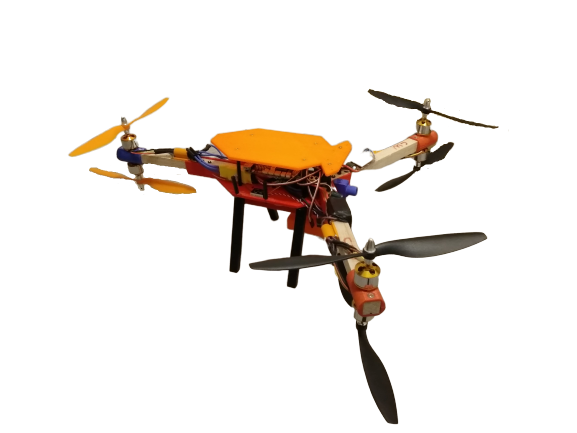
\includegraphics[width=0.8\linewidth]{Y6UAV1-removebg-preview.png}
			\caption{Y6 Hexarotor UAV}
			\label{fig:Y6Hexarotor}
		\end{figure}
		\space
		\subsection{UAV}
			The UAV under consideration throughout this project is an asymmetrical Y6 hexarotor. This kind of configuration has actuators in 3 counter-rotating co-axial pairs and 3 motor groups. A coaxial Y6 hexarotor is mechanically simpler than a classical helicopter since it has propellers with constant pitch and without a swash plate [6]. The advantages of Y6- hexarotors with respect to other multirotor configurations and classical helicopters is that the double drive configuration increases the thrust without increasing the frame size, while naturally eliminating the loss of efficiency due to torque compensation, another advantage of this configuration is better stability. However, the disadvantages are the higher energy consumption for six propulsion units and inefficiency due to the aerodynamic interaction present with co-axial actuator combinations[9]. The UAV is actuated by 6 1000Kv BLDC motors [14], attached to 6 10x45inch propellers and is powered by a 4-cell lithium-polymer battery. The exact details involved with the design, development and construction of UAVs is beyond the scope of the project investigation but material, mechanical and electronic consideration when designing such craft are explored in [12].
			
			\newpage
			
			\begin{figure}[h!]
				\centering
				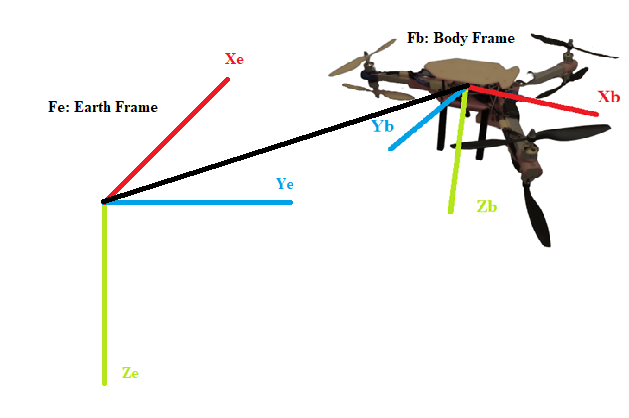
\includegraphics[width=0.7\linewidth]{UAVwithFrames.png}
				\caption{Coordinate Frames}
				\label{fig:Coordinate frames}
			\end{figure}
			
			Mathematical models are used to describes the characteristics of physical systems. They are derived from assumptions made about a systems behaviour which are represented abstractly using mathematics [3]. In modelling systems, it is first necessary to state all assumptions made about its characteristics. These assumptions simplify the process of model abstraction to ensure minimum viability standards are met. This allows for a mapping of multirotor movement and behaviour with the respect to it inputs and external influences. This means mathematical models can be considered as a series of functions that map inputs onto outputs while determining all the important time  dependant elements of the system, and as such, it is possible to predict the position and attitude of multirotors [3]. 
			\\ \\
			Following that, initially, multirotors can be defined as; rigid-bodies free to move in 3-D space with 6-DOF, with all motion restricted to being either rotational or translational.
			\\ \\
			More detailed mathematical models may describe certain multirotor characteristics more accurately, but they also require more computational resources which can lead to, longer simulation times, the inability to successfully complete simulations [5], and more complex than necessary control design processes and solutions.
			\\ \\
			This project will derive and present 2 models, a Non-linear model utilised in simulation, and a Linear model utilised in analysis and control design.
			
			\subsection{Kinematics}
			
				Multirotor mathematical models have to describe attitude and position according to the geometry of the UAV [6]. one of the most important parts of multirotor modelling is understanding the geometric and kinematic relationships between the reference frames [8]. Kinematics is the study of motion in terms of positions and velocities without regard to the forces causing the motion. Multirotor motion can be described by a number of variables called states, that are related and change with suitably chosen axes systems or reference frames [1]. These reference frames are:
				
				\begin{itemize}
					\item
						The Earth Frame: Fe
					\item 
						The Body Frame: Fb  
				\end{itemize}
				\space
				Each frame consists of 3 orthogonal axes, \(Xe,Ye,Ze\) and \(Xb,Yb,Zb\) respectively, about and along which rotational and translational motion respectively can occur. Where Fe is fixed to the earth near the multirotor such that a flat earth assumption can be made and sustained [2] and Fb is attached to the vehicle, centred at the UAV’s centre of mass, which is free to move with respect to Fe. The usual convention for the axes representation is to have a fixed right-handed axes system with the positive Z axes pointing downwards, towards the earth when levelled or hovering, the positive X axis pointing forward and the positive y axis pointing towards right or starboard side. This convention is referred to as the NORTH-EAST-DOWN Right-handed coordinate system [1],[2],[8]. Given the definition of the coordinate reference frames, system variables can now be defined in terms of these reference frames.
				\\ \\
				In the Fe, we define vectors:
				\\
				$$
				\vec{El} = 
				\begin{bmatrix}
					x \\
					y \\
					z
				\end{bmatrix}
				$$
				which represent the linear translational positions of Fb’s centre with respect to (w.r.t) Fe.
				\\
				$$
				\vec{Er} = 
				\begin{bmatrix}
					\phi \\
					\theta \\
					\psi
				\end{bmatrix}
				$$
				which represent the angular rotation of Fb about all 3 axes respectively, w.r.t Fe. Which are also known as (roll, pitch, yaw) respectively.
				\\
				In the Fb, we define vectors:
				\\
				$$
				\vec{Bl} = 
				\begin{bmatrix}
					u \\
					v \\
					w
				\end{bmatrix}
				$$
				which represents the linear velocity in each Fb axis respectively.
				\\
				$$
				\vec{Br} = 
				\begin{bmatrix}
					p \\
					q \\
					r
				\end{bmatrix}
				$$
				which represents the angular velocity in each Fb axis respectively.
				\\
				From these 12 elemental variables and 4 elemental vectors all, subsequent states and motion can be derived and represented [1][2][4].
				\\ \\
				Taking the \(\phi, \theta, \psi\) representation, the rotational motions of Fb w.r.t Fe can be derived by looking at rotations about each axis individually. Decomposing any arbitrary motion and orientation in 3-D Euclidean space in this manner presents a sequence of three elemental rotations of each axes of Fb w.r.t its counterpart in Fe. These elemental rotation angles are known as $\emph{Euler angles}$  and rotations are represented as direction cosine matrices [1],[2]. These are:
				\\
				$$
				R_\psi = 
				\begin{bmatrix}
					C_\psi & S_\psi & 0  \\
					-S_\psi & C_\psi & 0  \\
					0 & 0 & 1
				\end{bmatrix}
				$$
				\\
				$$
				R_\theta = 
				\begin{bmatrix}
					C_\theta & 0 & -S_\theta \\
					0 & 1 & 0 \\
					S_\theta & 0 & C_\theta
				\end{bmatrix}
				$$
				\\
				$$
				R_\phi = 
				\begin{bmatrix}
					1 & 0 & 0 \\
					0 & C_\phi & S_\phi  \\
					0 & -S_\phi & C_\phi
				\end{bmatrix}
				$$
				\space
				These elemental rotations can by combined using the ZYX convention which multiplies them together in the specific sequence:
				\[R_\psi \cdot R_\theta \cdot R_\phi\]
				to produce a matrix, the inverse of which, R, is able to map the translational motion of Fb unto Fe give any set of arbitrary \(\phi, \theta, \psi\) values. [1],[2],[3],[4],[5],[6],[7],[8],[9].
				\\
				$$
				R = 
				\begin{bmatrix}
					C_\theta C_\psi & -C_\theta S_\psi + S_\phi S_\theta C_\psi & -S_\phi S_\psi + C_\phi S_\theta C_\psi \\
					C_\theta S_\psi &  C_\phi C_\psi + S_\phi S_\theta S_\psi   & -S_\phi C_\psi + C_\phi S_\theta S_\psi \\
					-S_\theta       &  S_\phi C_\theta                          &  C_\phi C_\theta
				\end{bmatrix}
				$$
				\\
				Therefore: 
				\[ \dot{\vec{El}} = R \cdot \vec{Bl} \]
				\\
				Which maps the linear velocities and accelerations in Fb to linear velocities and accelerations with respect to Fe.
				\\
				Similarly, to map the angular velocities and accelerations in Fb w.r.t Fe requires another transformation matrix, the inverse of which, T, is also derived from the manipulation of Euler angles [1],[4]. 
				\\
				$$
				T = 
				\begin{bmatrix}
					1 & S_\phi T_\theta & C_\phi T_\theta \\
					0 & C_\phi & -S_\phi\\
					0 & \frac{S_\phi}{C_\theta}  & \frac{C_\phi}{C_\theta}
				\end{bmatrix}
				$$ 
				\\
				Therefore:
				\\
				\[\dot{\vec{Er}} = T \cdot \vec{Br} \]
				\\
				Where S, C, T, represent Sin, Cosine and Tan respectively.
				
			\subsection{Kinetics}
			
				Kinetics is the study of motion considering the forces and torques which cause the motion. As stated in the previous UAV subsection, the project looks at a Y6 hexarotor UAV which possesses 6 BLDC motors with propellers in a coaxial motor layout. Each motor propeller unit produces a thrust force, the collective effect of which can be summed and lumped together as a single force F, which means:
				\\
				\[\sum_{n = 1}^{n = 6}F_n\]
				\\
				where n denotes the motor index.
				\\
				Each motor propeller unit or propulsive unit, also produces a reaction torque. When a motor turns, in overcoming air resistance, a reactive force acts on the propeller in the direction opposite to the motor's rotation which produce a torque acting on the UAV body. These torques, $\tau$, can then also be summed together, meaning:
				\\
				\[\sum_{n = 1}^{n = 6}\tau_n\] 
				\\
				The co-axial configuration also ensures single point torque balancing [6]. meaning, so long as all rotors pair each produce the same torque, the net reactive torque produced is zero. The translational and angular motion of the Y6 hexarotor is controlled by thrust forces and torques produced by each motor. The main thrust is the sum of all rotors thrust, and rotational movement is generated by differences in individual  motor thrusts and torques [9].
				
				\subsection*{Newton-Euler}
				
					The Multirotor 6-DOF rigid body kinetics and takes into account the mass, and the inertia of the body. These are described by differential equations, which are derived through the utilization of the Newton-Euler modelling convention which derives representations of systems dynamics through the application of first principles via newtons 2nd law of motion aggregating all forces and torques applied to the rigid body by its actuators and environment while observing the resultant accelerations produced.
					\\
					Resolving the Forces acting linearly on the UAV:
					\\
					$$ 
					M 
					\begin{bmatrix}
						\ddot{x} \\
						\ddot{y} \\
						\ddot{z}
					\end{bmatrix}
					=
					M 
					\begin{bmatrix}
						0 \\
						0 \\
						g
					\end{bmatrix}
					-
					\begin{bmatrix}
						C_\theta C_\psi & -C_\theta S_\psi + S_\phi S_\theta C_\psi & -S_\phi S_\psi + C_\phi S_\theta C_\psi \\
						C_\theta S_\psi &  C_\phi C_\psi + S_\phi S_\theta S_\psi   & -S_\phi C_\psi + C_\phi S_\theta S_\psi \\
						-S_\theta       &  S_\phi C_\theta                          &  C_\phi C_\theta
					\end{bmatrix}
					\begin{bmatrix}
						\ddot{u} \\
						\ddot{v} \\
						\ddot{w} 
					\end{bmatrix}
					-
					\begin{bmatrix}
						D_lxx & 0 & 0 \\
						0 & D_lyy & 0 \\
						0 & 0 & D_lzz
					\end{bmatrix}
					\begin{bmatrix}
						\dot{x} \\
						\dot{y} \\
						\dot{z} 
					\end{bmatrix}
					$$ 
					\[ M \cdot \ddot{\vec{El}} = R \cdot \ddot{\vec{Bl}} - M \cdot \vec{g} - diag(D_l) \cdot \dot{\vec{El}}\] 
					where M is mass, g is acceleration due to gravity acting in the vertical Ze axis plane, and \(D_l\) is a diagonal matrix of drag coefficients with aerodynamic drag acting directly proportional to velocity in the Fe frame.
					\\
					Given that all thrust forces from the motor act along the same Zb axis plane, and there are no other force acting in the other axes therefore, the resultant equation can be rewritten as:
					\\
					$$ 
					M 
					\begin{bmatrix}
						\ddot{x} \\
						\ddot{y} \\
						\ddot{z}
					\end{bmatrix}
					=
					M 
					\begin{bmatrix}
						0 \\
						0 \\
						g
					\end{bmatrix}
					-
					\begin{bmatrix}
						C_\theta C_\psi & -C_\theta S_\psi + S_\phi S_\theta C_\psi & -S_\phi S_\psi + C_\phi S_\theta C_\psi \\
						C_\theta S_\psi &  C_\phi C_\psi + S_\phi S_\theta S_\psi   & -S_\phi C_\psi + C_\phi S_\theta S_\psi \\
						-S_\theta       &  S_\phi C_\theta                          &  C_\phi C_\theta
					\end{bmatrix}
					\begin{bmatrix}
						0 \\
						0 \\
						\sum F_n 
					\end{bmatrix}
					-
					\begin{bmatrix}
						D_lxx & 0 & 0 \\
						0 & D_1yy & 0 \\
						0 & 0 & D_lzz
					\end{bmatrix}
					\begin{bmatrix}
						\dot{x} \\
						\dot{y} \\
						\dot{z} 
					\end{bmatrix}
					$$ 
					\\
					Resolving the torques and forces acting angularly on the UAV in Fb:
					\\
					$$ 
					\begin{bmatrix}
						Ixx & 0 & 0 \\
						0 & Iyy & 0 \\
						0 & 0 & Izz
					\end{bmatrix} 
					\begin{bmatrix}
						\dot{p} \\
						\dot{q} \\
						\dot{r}
					\end{bmatrix}
					=
					\begin{bmatrix}
						A_p \\
						A_q \\
						A_r
					\end{bmatrix}
					-
					\begin{bmatrix}
						p \\
						q \\
						r 
					\end{bmatrix}
					\times
					\begin{bmatrix}
						Ixx & 0 & 0 \\
						0 & Iyy & 0 \\
						0 & 0 & Iyy
					\end{bmatrix}
					\begin{bmatrix}
						p \\
						q \\
						r 
					\end{bmatrix}
					-
					\begin{bmatrix}
						D_rxx & 0 & 0 \\
						0 & D_ryy & 0 \\
						0 & 0 & D_rzz
					\end{bmatrix}
					\begin{bmatrix}
						p \\
						q \\
						r
					\end{bmatrix}
					$$ 
					\[ I \cdot \dot{\vec{Br}} = A - C -  diag(D_r) \cdot \vec{Br}  \]
					\\
					Where A is the vector of torques generated by the sum of motor forces and torques in each axis, C is the Corriolis matrix formed of the cross product between the angular velocity vector and the diagonal inertia Tensor I, and \(D_r\) is the diagonal matrix of drag coefficients acting against motion in each axis.. 
					\\
					The A vector breaks down to:
					\\
					\[ A_p = L_1 ((F_1+F_2) - (F_3+F_4)) \]
					\\
					\[ A_q = L_2 ((F_1+F_2+F_3+F_4) - L_3 (F_5+F_6)) \]
					\\
					\[ A_r = \sum_{n = 1}^{n = 6}\tau_n \]
					Where L is the perpendicular distance from each motor group to the centre of mass.
					
					\subsection*{Inertia}
					
						\begin{figure}[h!]
							\centering
							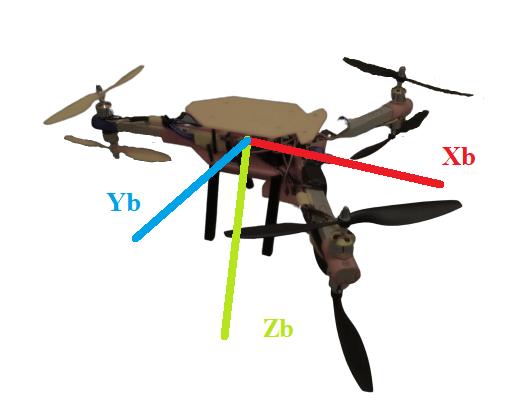
\includegraphics[width=0.6\linewidth]{UAVBodyFrame.png}
							\caption{UAV with Body Frame}
							\label{fig:uavbodyframe}
						\end{figure}
						
						Due to the asymmetry of the Y6 hexarotor, mass is not even distributed across the UAV frame. This creates a particular imbalance of inertia about the centre of mass, which is the centre of all rotation in Fb. This leads to a case where I has off diagonal elements[10]. i.e:
						\\
					    $$ 
						 I = 
						 \begin{bmatrix}
							 Ixx & Ixy & Ixy \\
							 Iyx & Iyy & Iyz \\
							 Izx & Izy & Izz
						 \end{bmatrix}
						$$
						 \\
						 This creates a situation whereby Fb as shown in Figure 5, is inaccurate and instead, is transposed to some other orientation, meaning rotation about the centre mass will occur in an oblong manner.
						 \\
						 To correct this, it is possible to adjust the inertia tensor by deriving some diagonalising operation such as performing an Eigen vector decomposition [10], this transformation will then need to be applied to all Inertia dependant terms in the angular motion calculation.
						 \\  
						 However, for the purpose of this investigation, it is possible to operate under the assumption that the system is symmetrical, as presented by a purely diagonal inertial tensor. This is due to the off-diagonal terms in the inertia matrix being far lower in magnitude than the diagonal terms themselves, meaning that the transposed reference frame does not differ too significantly from assumed symmetrical axes, thus any deviations can be reasonably neglected [10].
			
			\subsection{Actuator Dynamics}
			
				\begin{figure}[h!]
					\centering
					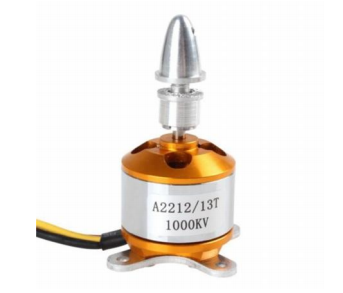
\includegraphics[width=0.4\linewidth]{BLDC.png}
					\caption{A2212/13T 1000KV BLDC Motor}
					\label{fig:BLDC}
				\end{figure}
				
				\begin{figure}[h!]
					\centering
					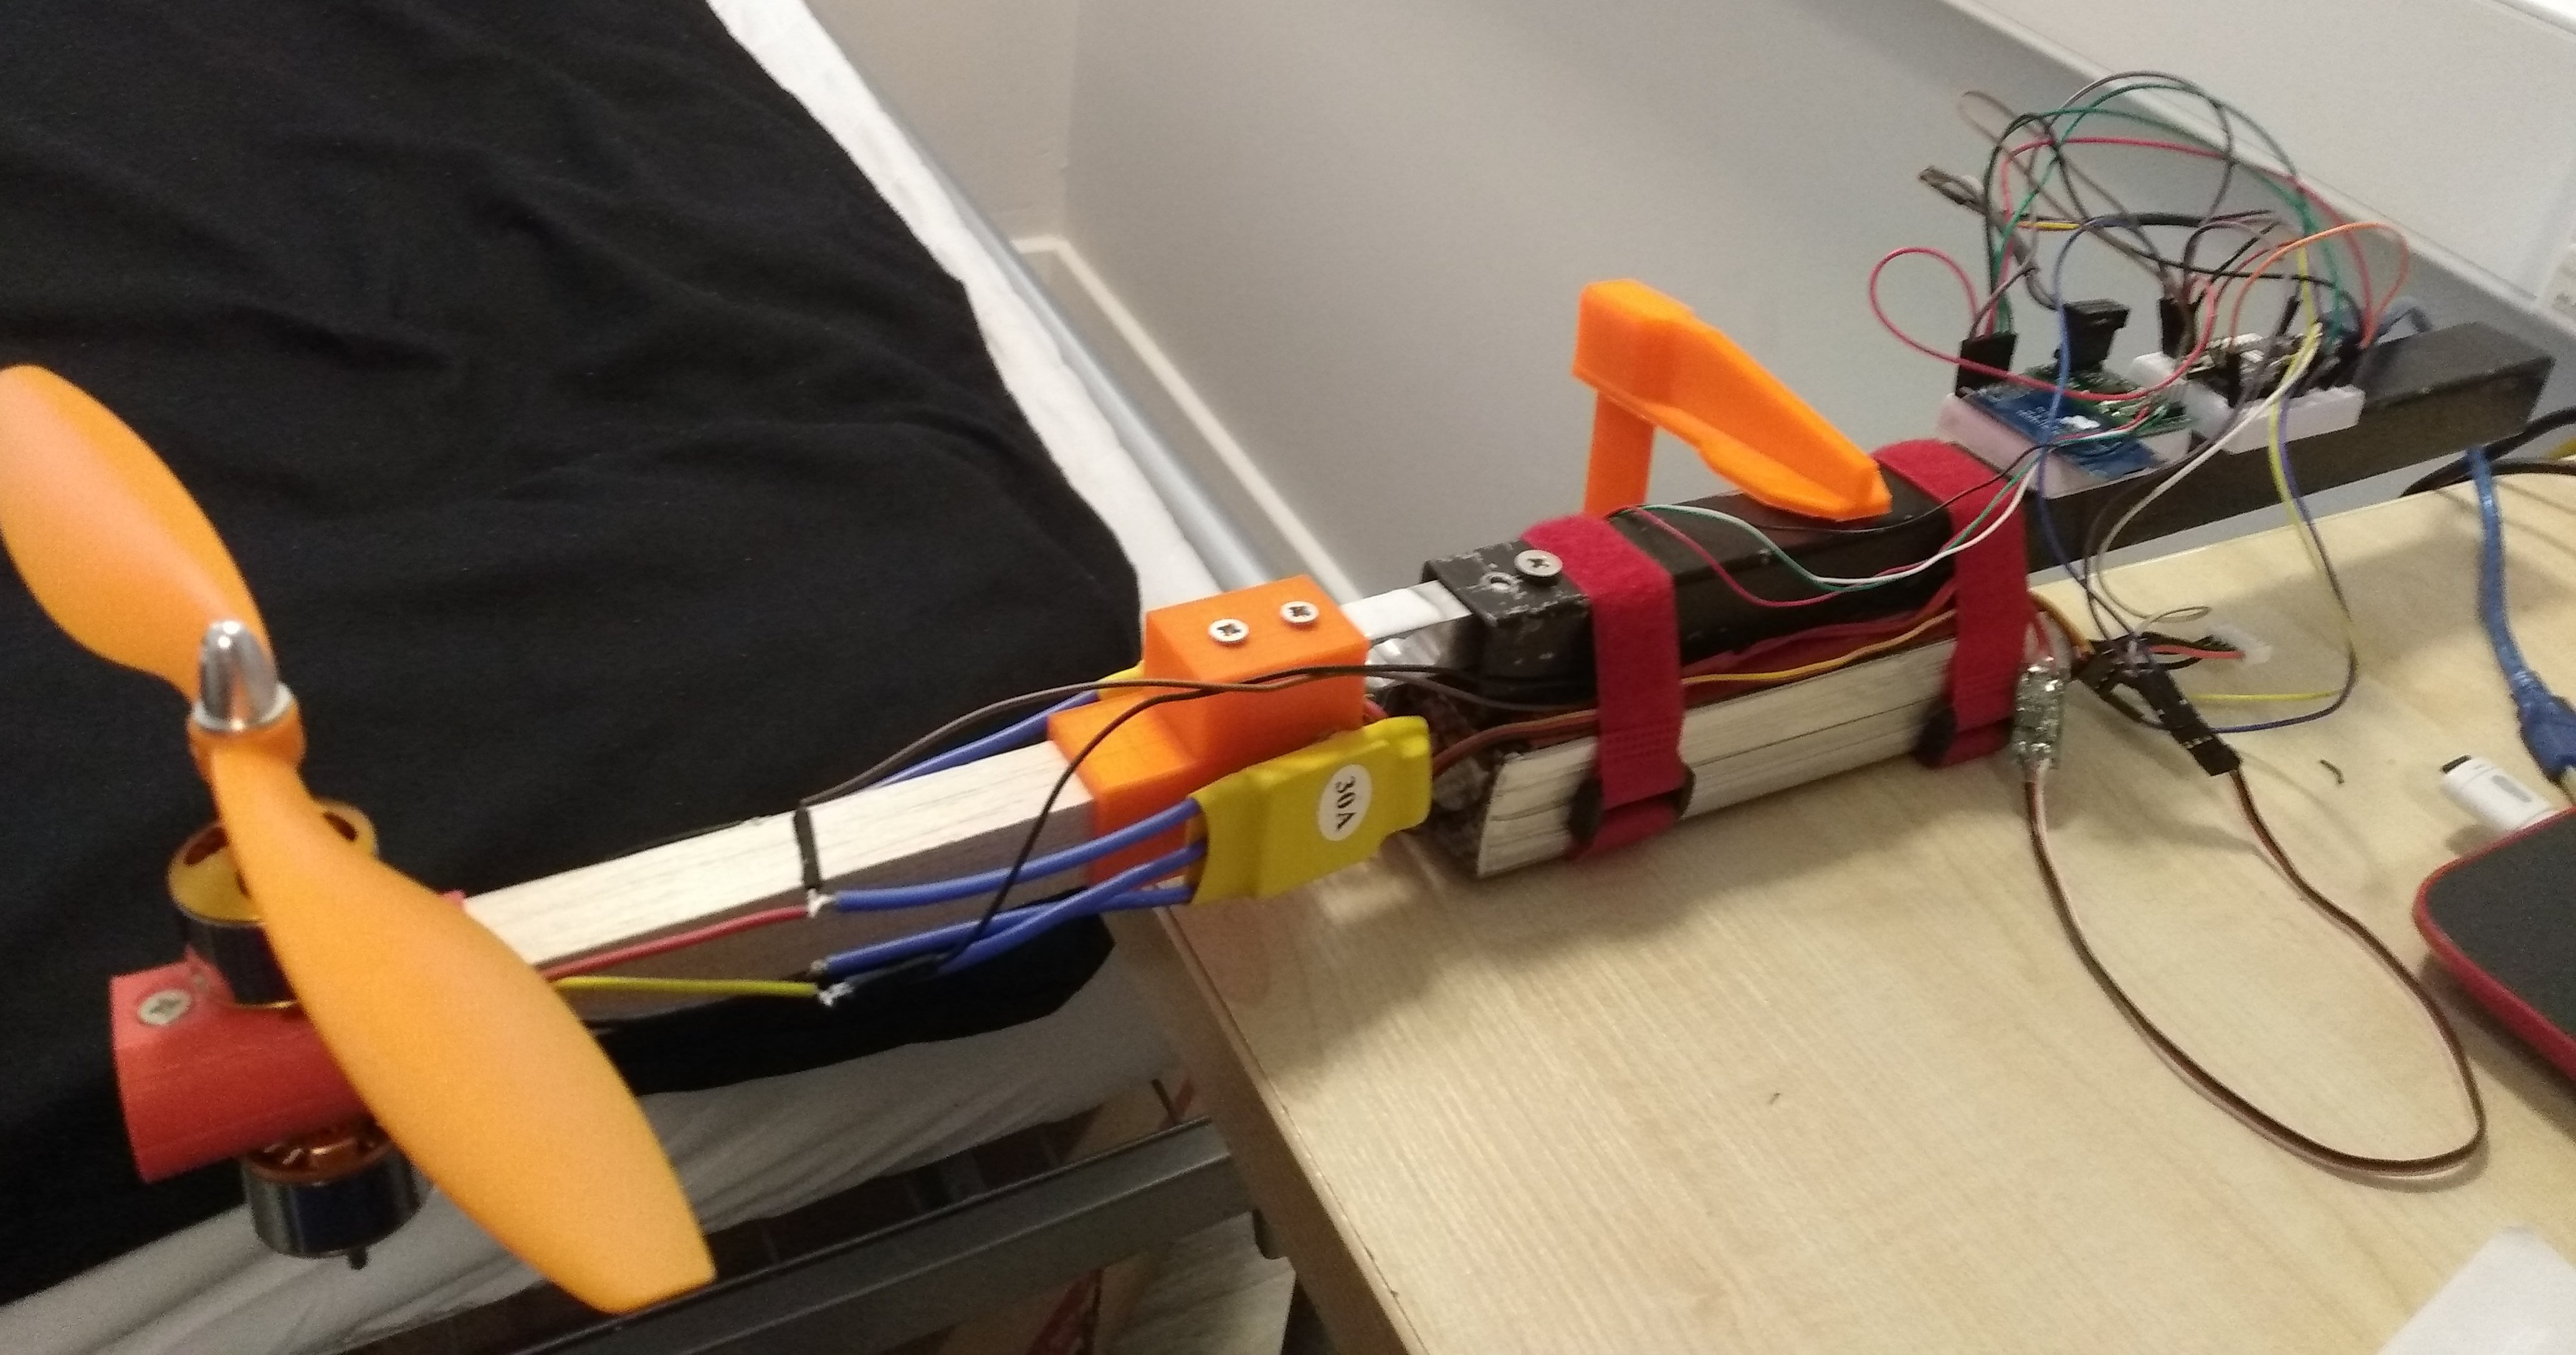
\includegraphics[width=0.5\linewidth]{TestStand1.jpg}
					\caption{Motor Test Stand}
					\label{fig:motorteststand}
				\end{figure}
				
				The thrust forces and torques acting on the multirotor UAV are primarily generated by propulsion units consisting of a BLDC motor, shown in Figure 6, an ECS and propeller. In order to produce a useful and fully developed systems model, the characteristics of the propulsive units must be known. This can either be done via first principles analysis looking at the mechanical, electrical and aerodynamic properties of each individual component, before calculating and then applying the results together in series to produce a high order, high fidelity model[17]. 
				\\ \\
				However taking this approach in many cases is unnecessary. This is due to being able to derive a lumped parameter model, which views the sum total of all the individual components as a single system with singular dynamics. Therefore, using system's response analysis and computational methods such as data fitting, it is possible via experimental systems identification to generate a lower order, minimum realisation model of sufficient fidelity [9],[12],[15],[16]. The systems identification approach involves the derivation of lumped parameter linear input-output models, between input PWM signal width and the output angular velocity, torque and thrust forces respectively using a motor test stand, shown in Figure 7, which consists of a load cell, for measuring forces and torques as well as an electronic revolutions per minute (RPM) sensor.
				\\
				\begin{figure}[h!]
					\centering
					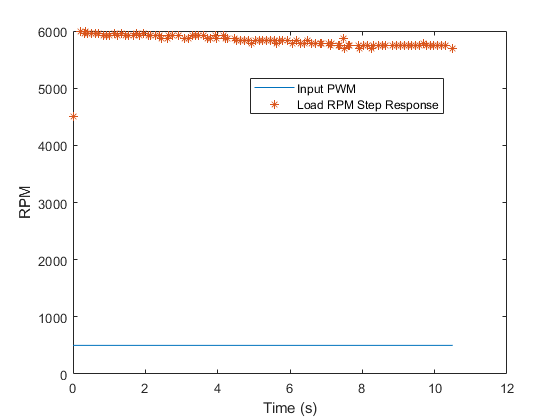
\includegraphics[width=0.8\linewidth]{InputStepData.png}
					\caption{Motor Input Step Data}
					\label{fig:inputstepdata}
				\end{figure}
				\\
				Using the Test stand, input-output PWM to RPM data is collected. Shown in Figure 8, is the response of the propulsive unit to a step input of 500$\mu s$. This data was then passed through the MATLAB system identification application where in order to account for potential delays in the input response, a first order transfer function model of the form:
				\\
				\[ \omega_n(s) = \frac{K_u}{\tau_m s + 1} \mu_n(s) \]
				\\
				is fit to the data where, $K_u$, is motor gain and $\tau_m$ is the response time constant, $\mu_n$ is the input PWM signal width and $\omega_n$ is the angular velocity. Figure 9 shows the response of the identified model to the same step of 500$\mu s$.
				\\
				This transfer function can then be reformulated into a differential equation
				\[\dot{\omega_n} = -\frac{1}{\tau_m}\omega_n	 + \frac{K_u}{\tau_m}\mu_n\]
				\\
				\begin{figure}[h!]
					\centering
					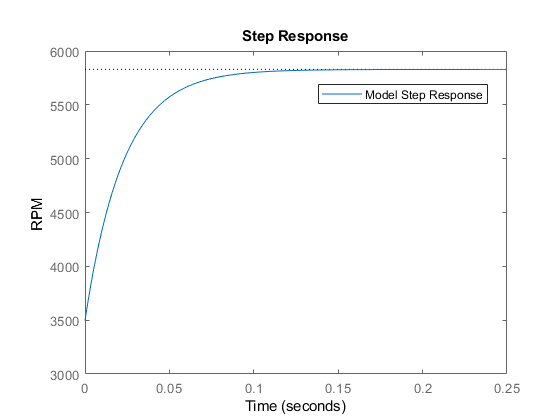
\includegraphics[width=0.8\linewidth]{ModelStep.png}
					\caption{First Order Model Step Response}
					\label{fig:modelstep}
				\end{figure}
				\\
				it is important to note that due to filtration present in the ESCs, the response time constant is sensitive to the frequency of the input PWM signal, therefore, throughout the investigation a frequency of 400 Hz is maintained.
				\\ \\
				Similarly, using the test stand, as shown in Figure 10 and Figure 11, data showing the relationship between the force and torque produced by the propulsion unit against generated angular velocity is shown. 2 quadratic models of the form: 
				\\
				\[ F_n = K_a \omega_n^2 + K_b\omega_n \]
				\[\tau_n = K_\tau \omega_n^2 \]
				\\
				respectively are then fit to the data where $\omega$ is the angular velocity of the motor, $K_a$, $K_b$ and $K_\tau$ are the force and torque coefficients respectively derived from the quadratic models.
				
				\newpage
				
				\begin{figure}[h!]
					\centering
					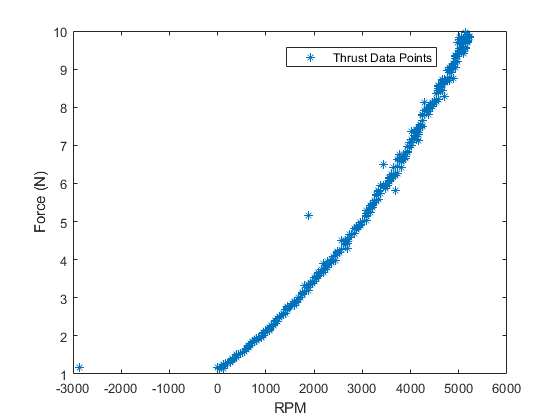
\includegraphics[width=0.8\linewidth]{ThrustData.png}
					\caption{Thrust against RPM}
					\label{fig:thrustdata}
				\end{figure}
				\begin{figure}[h!]
					\centering
					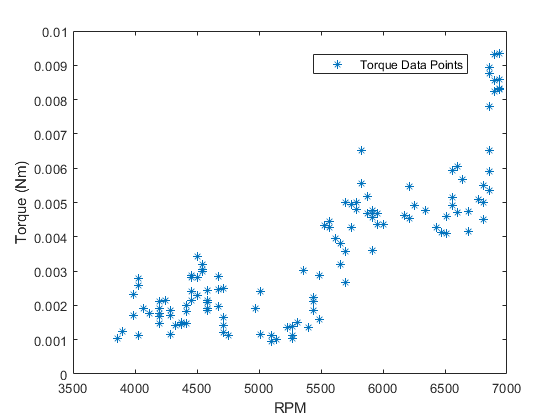
\includegraphics[width=0.8\linewidth]{TorqueData.png}
					\caption{Torque against RPM}
					\label{fig:torquedata}
				\end{figure}
			
			\newpage
			
			\subsection*{Non-Linear Model}
			
			Going through the modelling process presents the following non-linear mathematical model describing the dynamics of the Y6 hexarotor UAV. which will be used to produce a simulation of the system in MATLAB/Simulink.
			\\
			Translational Motion:
			\\ 
			$$ 
			M 
			\begin{bmatrix}
			\ddot{x} \\
			\ddot{y} \\
			\ddot{z}
			\end{bmatrix}
			=
			M 
			\begin{bmatrix}
			0 \\
			0 \\
			g
			\end{bmatrix}
			-
			\begin{bmatrix}
			C_\theta C_\psi & -C_\theta S_\psi + S_\phi S_\theta C_\psi & -S_\phi S_\psi + C_\phi S_\theta C_\psi \\
			C_\theta S_\psi &  C_\phi C_\psi + S_\phi S_\theta S_\psi   & -S_\phi C_\psi + C_\phi S_\theta S_\psi \\
			-S_\theta       &  S_\phi C_\theta                          &  C_\phi C_\theta
			\end{bmatrix}
			\begin{bmatrix}
			0 \\
			0 \\
			\sum F_n 
			\end{bmatrix}
			-
			\begin{bmatrix}
			D_lxx & 0 & 0 \\
			0 & D_1yy & 0 \\
			0 & 0 & D_lzz
			\end{bmatrix}
			\begin{bmatrix}
			\dot{x} \\
			\dot{y} \\
			\dot{z} 
			\end{bmatrix}
			$$ 
			\\
			Rotational Motion:
			\\
			$$ 
			\begin{bmatrix}
			Ixx & 0 & 0 \\
			0 & Iyy & 0 \\
			0 & 0 & Izz
			\end{bmatrix}
			\begin{bmatrix}
			\dot{p} \\
			\dot{q} \\
			\dot{r}
			\end{bmatrix}
			=
			\begin{bmatrix}
			A_p \\
			A_q \\
			A_r
			\end{bmatrix}
			-
			\begin{bmatrix}
			p \\
			q \\
			r 
			\end{bmatrix}
			\times
			\begin{bmatrix}
			Ixx & 0 & 0 \\
			0 & Iyy & 0 \\
			0 & 0 & Iyy
			\end{bmatrix}
			\begin{bmatrix}
			p \\
			q \\
			r 
			\end{bmatrix}
			-
			\begin{bmatrix}
			D_rxx & 0 & 0 \\
			0 & D_ryy & 0 \\
			0 & 0 & D_rzz
			\end{bmatrix}
			\begin{bmatrix}
			p \\
			q \\
			r
			\end{bmatrix}
			$$ 
			\\
			Where:
			\[ A_p = L_1 ((F_1+F_2) - (F_3+F_4)) \]
			\[ A_q = L_2 ((F_1+F_2+F_3+F_4) - L3 (F_5+F_6)) \]
			\[ A_r = \sum_{n = 1}^{n = 6}\tau_n \]
			and motor propulsion unit dynamics are:
			\[\dot{\omega_n} = -\frac{1}{\tau_m}\omega_n	 + \frac{K_u}{\tau_m}\mu_n\]
			\[ F_n = K_a \omega_n^2 + K_b\omega_n \]
			\[\tau_n = K_\tau \omega_n^2 \]
			\\
			Then applying \(\dot{\vec{Er}} = T \cdot \vec{Br} \) to convert angular velocity in Fb to angular velocity w.r.t Fe:
			\\
			$$
			\begin{bmatrix}
			\dot{\phi} \\
			\dot{\theta} \\
			\dot{\psi}
			\end{bmatrix}
			=
			\begin{bmatrix}
			1 & S_\phi T_\theta & C_\phi T_\theta \\
			0 & C_\phi & -S_\phi\\
			0 & \frac{S_\phi}{C_\theta}  & \frac{C_\phi}{C_\theta}
			\end{bmatrix}
			\begin{bmatrix}
			p \\
			q \\
			r 
			\end{bmatrix}
			$$ 
			
			\newpage
		
		\subsection{Linearisation}
				
			As with the UAV dynamics presented in the previous subsection, the majority of real world systems are non-linear, in that the states of the systems evolve in some fashion that does not satisfy the criteria for linearity. However, the majority of techniques developed over the decades in systems and control theory have been developed for application to and analysis of linear systems. Therefore in order to utilise these techniques in the presence of Non-linearities it is pertinent to devise some means, a least in a limited sense, of operating with Non-linear systems as if they were linear.[11] one means of accomplishing this is through the application of the  Jacobian process linearisation of non-linear systems about specific operating or equilibrium points.[11],[18]. First however, several assumptions need to be made to reduce the model complexity making it more amicable to linearisation. 
				
			\begin{enumerate}
				\item 
					The UAV is operating in stationary hover conditions
				\item 
					The effects of drag are negligible
				\item 
					Motor dynamics are purely quadratic
			\end{enumerate}

			Under these assumptions:
			\begin{itemize}
				\item
					$\ddot{\vec{Er}} \approx \dot{\vec{Br}} $
				\item
					C, $D_r$, and $D_l$ = 0
			\end{itemize}
			\space
			This reduces the model down to:
			$$ 
				M 
				\begin{bmatrix}
				\ddot{x} \\
				\ddot{y} \\
				\ddot{z}
				\end{bmatrix}
				=
				M 
				\begin{bmatrix}
				0 \\
				0 \\
				g
				\end{bmatrix}
				-
				\begin{bmatrix}
				C_\theta C_\psi & -C_\theta S_\psi + S_\phi S_\theta C_\psi & -S_\phi S_\psi + C_\phi S_\theta C_\psi \\
				C_\theta S_\psi &  C_\phi C_\psi + S_\phi S_\theta S_\psi   & -S_\phi C_\psi + C_\phi S_\theta S_\psi \\
				-S_\theta       &  S_\phi C_\theta                          &  C_\phi C_\theta
				\end{bmatrix}
				\begin{bmatrix}
				0 \\
				0 \\
				\sum F_n 
				\end{bmatrix}
			$$
			$$ 
				\begin{bmatrix}
				Ixx & 0 & 0 \\
				0 & Iyy & 0 \\
				0 & 0 & Izz
				\end{bmatrix}
				\begin{bmatrix}
				\ddot{\phi} \\
				\ddot{\theta} \\
				\ddot{\psi}
				\end{bmatrix}
				=
				\begin{bmatrix}
				L_1 ((F_1+F_2) - (F_3+F_4)) \\
				L_2 ((F_1+F_2+F_3+F_4) - L3 (F_5+F_6)) \\
				\sum_{n = 1}^{n = 6}\tau_n
				\end{bmatrix}
			$$ 
				\[\dot{\omega_n} = -\frac{1}{\tau_m}\omega_n	 + \frac{K_u}{\tau_m}\mu_n\]
				\[ F_n = K_a \omega_n^2\]
				\[\tau_n = K_\tau \omega_n^2 \]
				\\
				Multiplying out the matrices and collecting terms produces 6 distinct 2nd order non-linear Differential and 1 linear differential equation replicated for each motor representing the motor dynamics:
				\\
				\[\ddot{x} = \frac{\sum_{n=1}^{n=6}K_a \omega_n^2}{M}C\phi S\theta C\psi  + \frac{\sum_{n=1}^{n=6}K_a \omega_n^2}{M}S\phi S\psi \]
				\[\ddot{y} = \frac{\sum_{n=1}^{n=6}K_a \omega_n^2}{M}C\phi S\theta C\psi  - \frac{\sum_{n=1}^{n=6}K_a \omega_n^2}{M}S\phi C\psi \]
				\[\ddot{z} = g - \frac{\sum_{n=1}^{n=6}K_a \omega_n^2}{M}C\phi C\theta \]
				\[\ddot{\phi} = \frac{L_1}{Ixx} ((K_a \omega_1^2+K_a \omega_2^2 +) - (K_a \omega_3^2+K_a \omega_4^2)) \]
				\[\ddot{\theta} = \frac{L_2}{Iyy} ((K_a \omega_1^2+K_a \omega_2^2+K_a \omega_3^2+K_a \omega_4^2) - \frac{L3}{Iyy} (K_a \omega_5^2+K_a \omega_6^2)) \]
				\[\ddot{\psi} = \frac{\sum_{n = 1}^{n = 6}K_\tau \omega_n^2}{Izz} \]
				\[\dot{\omega_n} = -\frac{1}{\tau_m}\omega_n	 + \frac{K_u}{\tau_m}\mu_n\]
				
				Here we can define the full state vector:
				$$
				X =
				\begin{bmatrix}
					x,\dot{x},y,\dot{y},z,\dot{z},\phi,\dot{\phi},\theta,\dot{\theta},\psi,\dot{\psi},\omega_1,\omega_2,\omega_3,\omega_4,\omega_5,\omega_6
				\end{bmatrix}
				$$
				However for the purposes of this project the full state isn't utilised as feedback control authority in x and y are not required to maintain a stable hover. therefore, a reduced state can be defined: 
				$$
				X =
				\begin{bmatrix}
				z,\dot{z},\phi,\dot{\phi},\theta,\dot{\theta},\psi,\dot{\psi},\omega_1,\omega_2,\omega_3,\omega_4,\omega_5,\omega_6
				\end{bmatrix}
				$$
				
				\subsection*{Jacobian Linearisation}
					
					In order to linearise the system equations, equilibrium points must be defined. These are the set of states and input values for which the system is stationary i.e:
					\[\dot{X} = f(X_e,\mu_e) = 0\]
					where f represents the systems dynamics,therefore, the following equilibrium input and state vectors can be defined:
					$$
					X_e = 
					\begin{bmatrix}
						1.5,0,0,0,0,0,0,0,\omega_e1,\omega_e2,\omega_e3,\omega_e4,\omega_e5,\omega_e6
					\end{bmatrix}
					$$
					$$
					\mu_e = 
					\begin{bmatrix}
						\mu_e1,\mu_e1,\mu_e1,\mu_e1,\mu_e1,\mu_e1
					\end{bmatrix}
					$$
					Following this, the system states are redefined in terms of deviations from these equilibrium points:
					\[\bar{X} = X - X_e\] 
					\[\bar{\mu} = \mu - \mu_e\] 
					These deviation variables are then substituted back into the dynamics equations and a first order Taylor's series expansion is performed. where:
					\[
						\dot{\bar{X}} = f(\bar{X},\bar{\mu}) + \frac{\partial f}{\partial X}\bigg\vert_{\mu = \mu_e}^{X = X_e} + \frac{\partial f}{\partial \mu}\bigg\vert_{\mu = \mu_e}^{X = X_e}
					\]
					and:
					\[ f(\bar{X},\bar{\mu_e}) = 0 \]
					These differential equations approximately govern the deviation variables, and as long as they remain small, this presents a linear, time-invariant, differential equation, as the derivatives of $\bar{X}$ are now linear combinations of the deviation states and the deviation inputs, $\bar{\mu}$ [11]. 
					\\
					Finally, the Linear State-Space model emerges following:
					\\
					\[
						A = \frac{\partial f}{\partial X}\bigg\vert_{\mu = \mu_e}^{X = X_e}, \in R ^{n\times n}
					\] 
					\\
					\[ 
						B = \frac{\partial f}{\partial \mu}\bigg\vert_{\mu = \mu_e}^{X = X_e} , \in R ^{n\times m}
					\]
					Where n is the number of states, m the number of inputs, A the n-by-n dynamics matrix and B the n-by-m input matrix.
					\\ \\
					Thus:
					\\
					\setcounter{MaxMatrixCols}{15}
					A = 
					$$
					\begin{bmatrix}
						0&1&0&0&0&0&0&0&0&0&0&0&0&0\\
						0&0&0&0&0&0&0&0&\frac{2K_a\omega_e1}{M}&\frac{2K_wK_a\omega_e2}{M}&\frac{2K_a\omega_e3}{M}&\frac{2KwKa\omega_e4}{M}&\frac{2KwKa\omega_e5}{M}&\frac{2KwKa\omega_e6}{M}\\
						0&0&0&1&0&0&0&0&0&0&0&0&0&0\\
						0&0&0&0&0&0&0&0&\frac{2L_1Kthrust\omega_e1}{Ixx}&\frac{2L_1K_wK_a\omega_e2}{Ixx}& \frac{-2L_1K_a\omega_e3}{Ixx}&\frac{-2L_1K_wK_a\omega_e4}{Ixx}&0&0\\
						0&0&0&0&0&1&0&0&0&0&0&0&0&0\\
						0&0&0&0&0&0&0&0&\frac{2L_1K_a*\omega_e}{Iyy}&\frac{2L_2K_wK_a\omega_e2}{Iyy}& \frac{2L_2K_a\omega_e3}{Iyy}&\frac{2L_2K_wK_a\omega_4}{Iyy}&\frac{-2L_3K_a*\omega_e5}{Iyy}&\frac{-2L_3K_wK_a\omega_e6}{Iyy}\\
						0&0&0&0&0&0&0&1&0&0&0&0&0&0\\
						0&0&0&0&0&0&0&0&\frac{-2K_\tau\omega_e1}{Izz}&\frac{2K_\tau\omega_e2}{Izz}&\frac{2K_\tau\omega_e3}{Izz}&\frac{-2K_\tau\omega_e4}{Izz}&\frac{-2K_\tau\omega_e5}{Izz}&\frac{2K_\tau\omega_e6}{Izz}\\
						0&0&0&0&0&0&0&0&\frac{-1}{\tau_m}&0&0&0&0&0\\
						0&0&0&0&0&0&0&0&0&\frac{-1}{\tau_m}&0&0&0&0\\
						0&0&0&0&0&0&0&0&0&0&\frac{-1}{\tau_m}&0&0&0\\
						0&0&0&0&0&0&0&0&0&0&0&\frac{-1}{\tau_m}&0&0\\
						0&0&0&0&0&0&0&0&0&0&0&0&\frac{-1}{\tau_m}&0\\
						0&0&0&0&0&0&0&0&0&0&0&0&0&\frac{-1}{\tau_m}
					\end{bmatrix}
					$$
					\\
					B = 
					$$
					\begin{bmatrix}
					0&0&0&0&0&0\\
					0&0&0&0&0&0\\
					0&0&0&0&0&0\\
					0&0&0&0&0&0\\
					0&0&0&0&0&0\\
					0&0&0&0&0&0\\
					0&0&0&0&0&0\\
					0&0&0&0&0&0\\
					\frac{K_u}{Mtau}&0&0&0&0&0\\
					0&\frac{K_u}{Mtau}&0&0&0&0\\
					0&0&\frac{K_u}{Mtau}&0&0&0\\
					0&0&0&\frac{K_u}{Mtau}&0&0\\
					0&0&0&0&\frac{K_u}{Mtau}&0\\
					0&0&0&0&0&\frac{K_u}{Mtau}
					\end{bmatrix}
					$$
			\newpage
			
			\begin{tabular}{ |p{2cm}||p{10cm}|p{3cm}|p{3cm}|  }
				\hline
				\multicolumn{3}{|c|}{Model Parameters} \\
				\hline
				Character& Name  & Value  \\
				\hline
				F        &  Thrust Force                                         & AFG\\
				$\tau$   &  Torque                                               & ALA\\
				M        &  Mass                                                 & ALB\\
				Ixx      &  Inertia about Xb                                     & DZA\\
				Iyy      &  Inertia about Yb                                     & ASM\\
				Izz      &  Inertia about Zb                                     & AND\\
				$D_lxx$  &  Translational Drag Coefficient in Xe                 & AGO\\
				$D_lyy$  &  Translational Drag Coefficient in Ye                 & AGO\\
				$D_lzz$  &  Translational Drag Coefficient in Ze                 & AGO\\
				$D_rxx$  &  Angular Drag Coefficient in Xb                       & AGO\\
				$D_ryy$  &  Angular Drag Coefficient in Yb                       & AGO\\
				$D_rzz$  &  Angular Drag Coefficient in Zb                       & AGO\\
				$L_1$    &  Lateral Length From Motor 1 To Center Of Mass        & AGO\\
				$L_2$    &  Longitudinal Length From Motor 1 To Center Of Mass   & AGO\\
				$L_3$    &  Longitudinal Length From Motor 5 To Center Of Mass   & AGO\\
				$K_u$    &  Motor RPM Gain                                       & AGO\\
				$\tau_m$ &  Motor RPM Time Constant                              & AGO\\
				$K_a$    &  Quadratic RPM to Force Gain                          & AGO\\
				$K_b$    &  Linear RPM to Force Gain                             & AGO\\
				$K_\tau$ &  Quadratic RPM to Torque Gain                         & AGO\\
				\hline
			\end{tabular}
			
			\newpage
	\section{Linear Quadratic Gaussian Control}
		
		\newpage
						
	%\bibliographystyle{plain}			
	%\bibliography{ProjectResearchPapers}
				
\end{document}